\documentclass[tikz, margin=3mm]{standalone}
\usetikzlibrary{fit,
                positioning,
                shapes}
\newcounter{nodeno}
\begin{document}
    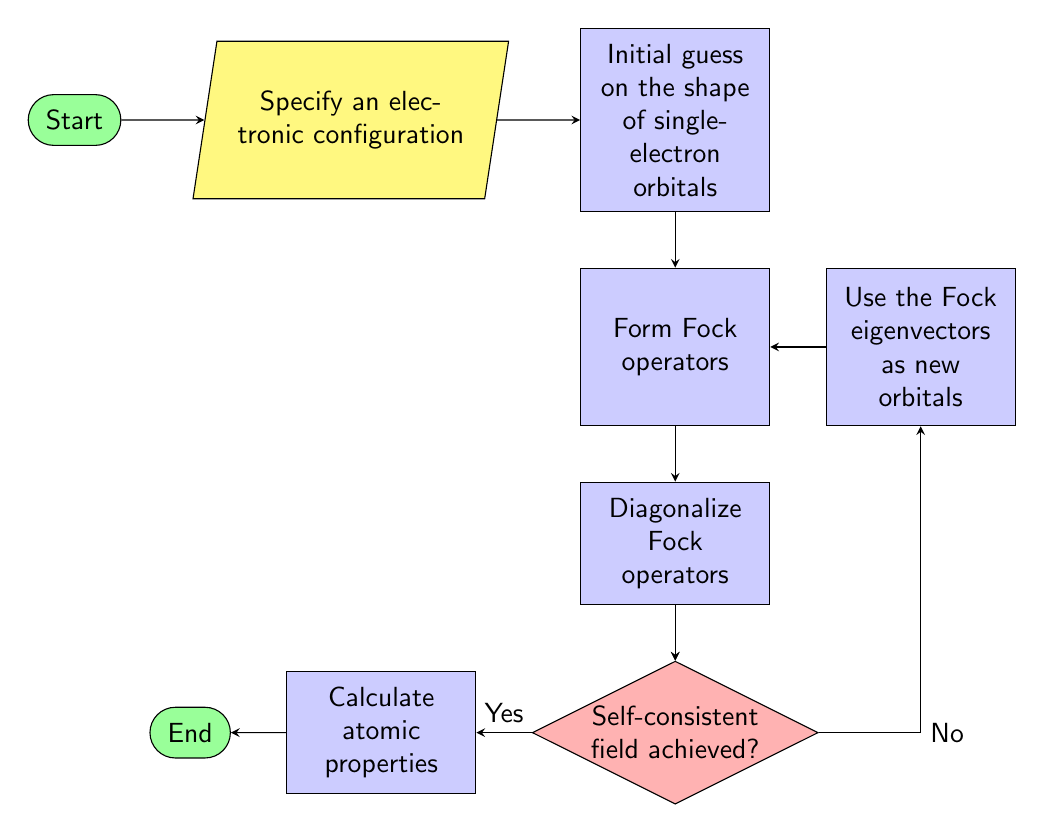
\begin{tikzpicture}[node font=\sffamily,
    stepnodeno/.code=\stepcounter{nodeno},
    every node/.append style={stepnodeno,
        alias=LN-\number\value{nodeno}},
     a/.style={above=#1 of LN-\the\numexpr\value{nodeno}-1},
     b/.style={below=#1 of LN-\the\numexpr\value{nodeno}-1},
     r/.style={right=#1 of LN-\the\numexpr\value{nodeno}-1},
     l/.style={left=#1 of LN-\the\numexpr\value{nodeno}-1},
     a/.default=2em,b/.default=2em,l/.default=2em,r/.default=2em,
     base/.style = {draw, align=center, 
                    inner sep=2mm%, on chain=A, join=by arr
                    },
startstop/.style = {base, rounded rectangle,fill=green!40},
      io/.style = {base, text width=3cm, trapezium, trapezium stretches body,
                    trapezium left angle=75, trapezium right angle=105,fill=yellow!50},
  process/.style = {base, text width=2cm, minimum height=1cm,fill=blue!20},
 decision/.style = {base, text width=2.5cm, diamond, aspect=2, inner xsep=-5mm,align=center,fill=red!30},
      arr/.style = {-stealth},
      task/.style={process,name=DT#1},
      output/.style={rectangle,path picture={
        \draw ([xshift=-\pgflinewidth/2,yshift=\pgflinewidth/2]path picture bounding box.south east)
        -| ([xshift=\pgflinewidth/2,yshift=-\pgflinewidth/2]path picture bounding box.north west) 
        --
        ([xshift=-1em,yshift=-\pgflinewidth/2]path picture bounding box.north east)
        --
        ([xshift=-\pgflinewidth/2,yshift=-1em]path picture bounding box.north east)
        -- cycle; },minimum width=1.5cm,minimum height=1cm},
      node distance = 2em and 2em]
\node[startstop] (Start) {Start};                        
\node[r=3em,io,minimum height=2cm] (S) {Specify an electronic configuration};
\node[r=3em,task=1,minimum height=2cm]  {Initial guess on the shape of single-electron orbitals};
\node[b,task=2,minimum height=2cm]  {Form Fock operators};
\node[b,task=3] {Diagonalize Fock operators}; 
\node[b,decision] (C1) {Self-consistent field achieved?};
%\node[b=4em,task=10] {};
%\node[b=4em,task=9] {};
%\node[l=5em,task=8] {};
%\node[a,task=7,minimum height=1.5cm] {};
%\node[a,task=6,minimum width=3.5cm] {};
%\node[l,task=5,minimum height=1.5cm] {};
\node[l,task=4] {Calculate atomic properties};
%\node[right=of C1,decision] (C2) {Cond\\ 2};
\node[l,startstop] (End) {End};
\node[right=of DT2,task=5,minimum height=2cm]  {Use the Fock eigenvectors as new orbitals};
\foreach \X in {1,...,4}
{\draw[arr] (LN-\X) -- (LN-\the\numexpr\X+1);}
%\foreach \X in {5,...,11}
%{\draw[arr] (LN-\the\numexpr\X+1) -- (LN-\X);}
%\draw[arr] (C1) -- node[above] (Y1) {Yes}(C2);
%\draw[arr] (C2) |- node[left,pos=0.25] (N1) {No}(DT9);
%\draw[arr] (C2) -- node[left] (Y2) {Yes}(out);
\draw[arr] (DT4) -- (End);
\draw[arr] (DT3) -- (C1);
\draw[arr] (DT3) -- (C1);
\draw[arr] (DT5) -- (DT2);
\draw[arr] (C1) -| node[right,pos=0.5] (N2) {No}(DT5);
\draw[arr] (C1) -- node[above,pos=0.5] (N2) {Yes}(DT4);
\end{tikzpicture}
\end{document}